\documentclass[12pt,a4paper]{article}

\usepackage[a4paper,margin=1in]{geometry}
\usepackage{graphicx}
\usepackage{booktabs}
\usepackage{amsmath,amssymb}
\usepackage{float}
\usepackage{hyperref}
\usepackage{xcolor}
\usepackage{listings}
\usepackage{enumitem}
\usepackage{fancyhdr}
\usepackage{longtable}
\usepackage{subcaption}   % required for the 2-graphs-per-row layout
\usepackage{mathptmx}     % Times New Roman substitute font (text + math)
\usepackage{fontawesome} % for using icons

\hypersetup{colorlinks=true,linkcolor=blue,urlcolor=blue}

\pagestyle{fancy}
\fancyhf{}
\lhead{ICS1512}
\rhead{Machine Learning Algorithms Laboratory}
\cfoot{\thepage}

\lstset{
language=Python,
basicstyle=\ttfamily\small,
numbers=left,
frame=single,
breaklines=true,
showstringspaces=false
}

\begin{document}

\begin{tabular}{|p{4cm}|p{11cm}|}
\hline
Experiment No. & 5\\ \hline
Experiment Title &  Decision Tree and Random Forest: A Comparative Classification Study \href{https://github.com/Poojashree81/ICS1512-Machine-Learning-Laboratory.git}{\faGithub} \\ \hline
Student Name & Poojashree V \\ \hline
Register Number & 3122247001043 \\ \hline
Faculty & Dr. Poreddy Ajay Kumar Reddy \\ \hline
Submission Date & 11th August 2026\\ \hline
\end{tabular}

\section{Objective}
\begin{itemize}[nosep]
\item Build a Decision Tree classifier that can separate malignant and benign tumours using the Wisconsin Diagnostic Breast Cancer (WDBC) measurements.
\item Extend the single tree into a Random Forest ensemble, and check whether bagging plus feature-subsampling actually reduces the variance we saw in the standalone tree.
\item Get a feel for how depth-related hyperparameters push each model toward overfitting on one end and underfitting on the other.
\item Pick hyperparameters using 5-Fold Cross-Validation instead of just eyeballing test-set performance, to keep the selection process honest.
\item Compare the tuned Decision Tree against the tuned Random Forest on the same train/test split, using Accuracy, Precision, Recall, F1-score and ROC-AUC.
\end{itemize}

\section{Problem Statement}
Breast cancer diagnosis from digitized fine needle aspirate (FNA) images can be framed as a binary classification problem. Given 30 numeric features that describe the size, shape and texture of cell nuclei, the task is to predict whether a tumour is \textbf{Malignant} or \textbf{Benign}. The input here is a $569 \times 30$ feature matrix and the output is a binary diagnosis label. Ideally the classifier should catch as many malignant cases as possible (high Recall) without flooding the output with false alarms (low Precision loss) -- in a clinical setting, both a missed cancer and an unnecessary scare carry real cost.

\section{Dataset Description}
\begin{longtable}{|p{6cm}|p{8cm}|}
\hline
Dataset Name & Wisconsin Diagnostic Breast Cancer (WDBC) Dataset \\
\hline
Dataset Source & UCI Machine Learning Repository (loaded via a Kaggle mirror: \texttt{poojashree81/breast-cancer-wisconsin}, file \texttt{wdbc.data}) \\
\hline
Number of Samples & 569 \\
\hline
Number of Features & 30 numerical attributes (10 base measurements $\times$ 3 statistics: mean, standard error, worst) \\
\hline
Number of Classes & 2 --- Malignant (M): 212 samples, Benign (B): 357 samples \\
\hline
Missing Values & None. \texttt{df.info()} reported 569 non-null entries for every one of the 32 columns (id, diagnosis + 30 features). \\
\hline
Train-Test Split & 80--20 stratified split $\rightarrow$ 455 training samples, 114 testing samples (\texttt{random\_state=42}) \\
\hline
\end{longtable}

\section{Exploratory Data Analysis}
\begin{figure}[H]
\centering

\includegraphics[width=0.62\linewidth]{figures/class_distribution.eps}
\caption{Class distribution of the WDBC dataset.}
\label{fig:class_dist}
\end{figure}
\textbf{Inference:} From Figure~\ref{fig:class_dist} we can see the dataset leans toward Benign -- 357 samples (62.7\%) against 212 Malignant (37.3\%), roughly a 1.68:1 split. That's not extreme enough to justify pulling in SMOTE or undersampling, but it's still enough of a skew that we used \texttt{stratify=y} when splitting, so both classes keep their original proportions in the train and test sets. It also explains why accuracy alone wasn't good enough here -- a model that just leans toward predicting Benign by default could still post a misleadingly high accuracy score, which is why Precision, Recall and F1 were tracked alongside it.
 
\begin{figure}[H]
\centering
\includegraphics[width=0.92\linewidth]{figures/feature_correlation.eps}
\caption{Pairwise Pearson correlation matrix across all 30 features.}
\label{fig:corr}
\end{figure}
\textbf{Inference:} Looking at Figure~\ref{fig:corr}, the \texttt{mean}, \texttt{se}, and \texttt{worst} groups of \{radius, perimeter, area\} form three tight, dark-red blocks (correlation roughly 0.96--1.0) -- radius, perimeter and area are, for the most part, three different ways of saying the same thing about tumour size. \texttt{concavity}, \texttt{concave points} and \texttt{compactness} cluster together too, which makes sense since all three are describing how irregular the cell boundary is. \texttt{smoothness} and \texttt{fractal\_dimension} stand apart from the size-based features (they show up as the paler, blue-ish cells), so they're probably contributing more independent information than the rest. This kind of multicollinearity doesn't really hurt tree-based models -- a split just latches onto one of the correlated features and ignores the others -- but it would be a bigger issue for something like a linear or distance-based classifier.
 

\section{Data Preprocessing}

\begin{itemize}
    \item \textbf{Missing value handling:} Not needed here -- the WDBC dataset came in complete, which \texttt{df.info()} confirmed.
    \item \textbf{Encoding:} We dropped the \texttt{id} column since it's just a non-predictive identifier. The target was remapped from the raw \texttt{M}/\texttt{B} codes to \texttt{Malignant}/\texttt{Benign} labels using \texttt{y = df["diagnosis"].map(\{...\})}, mostly for readability.
    \item \textbf{Feature scaling:} Skipped on purpose. Decision Trees and Random Forests split on threshold comparisons per feature, so they don't care about monotonic rescaling -- standardising the data wouldn't have changed a single split.
    \item \textbf{Train-test split:} 80--20 split via \texttt{train\_test\_split(..., stratify=y, random\_state=42)}, which keeps the 62.7/37.3 class ratio in both partitions (114 test samples work out to 42 Malignant, 72 Benign).
    \item \textbf{Feature engineering:} None -- all 30 raw features went in as-is.
\end{itemize}

\section{Machine Learning Algorithm}
\subsection*{Decision Tree Classifier}
A Decision Tree recursively splits the feature space, picking at each node the feature and threshold that cuts class impurity down the most. The two impurity criteria explored here were:
\[
\text{Gini}(t) = 1 - \sum_{i=1}^{C} p_i^2, \qquad
\text{Entropy}(t) = -\sum_{i=1}^{C} p_i \log_2(p_i)
\]
where $p_i$ is the proportion of class $i$ samples sitting at node $t$. Splitting keeps going until a stopping condition kicks in -- \texttt{max\_depth}, \texttt{min\_samples\_split}, or \texttt{min\_samples\_leaf}.
On the plus side, a Decision Tree is easy to interpret, doesn't need scaling, and can pick up non-linear interactions on its own. The downside is variance: a single tree is sensitive to small changes in the training data, and if you don't constrain it, it will happily memorise the training set instead of generalising.
 
\subsection*{Random Forest Classifier}
A Random Forest trains $B$ decision trees, each on a bootstrap resample of the training data, and additionally restricts each split to a random subset of \texttt{max\_features}. The final prediction is just a majority vote across the trees:
\[
\hat{y} = \text{mode}\{h_1(x), h_2(x), \dots, h_B(x)\}
\]
where $h_b$ is the $b$-th bootstrapped tree. Since the trees are decorrelated (through bagging plus random feature selection), averaging their votes brings the variance down without adding much bias -- this is the classical bagging argument from Breiman (2001), and it's more or less what we ended up observing in this experiment too. The trade-off is that a forest loses the single-tree's interpretability and costs more to train and run.

\section{Experimental Setup}
\begin{tabular}{ll}
\toprule
Python Version & 3.12.13 \\
Scikit-Learn Version & \textit{[not printed in the notebook -- run \texttt{import sklearn; print(sklearn.\_\_version\_\_)} and fill in]} \\
IDE & Kaggle Notebook (Jupyter interface) \\
Operating System & Linux (Kaggle \texttt{kaggle/python} Docker image) \\
Hardware & CPU only -- no GPU/accelerator used (\texttt{isGpuEnabled: false} in notebook metadata) \\
\bottomrule
\end{tabular}


\section{Hyperparameter Selection}

Both models were tuned with \texttt{GridSearchCV} over a \texttt{StratifiedKFold(n\_splits=5, shuffle=True, random\_state=42)}, scoring on accuracy.
 
\begin{tabular}{ll}
\toprule
Parameter & Value \\
\midrule
\multicolumn{2}{l}{\textit{Decision Tree (best combination, CV Accuracy = 92.97\%)}} \\
criterion & gini \\
max\_depth & 7 \\
min\_samples\_split & 5 \\
min\_samples\_leaf & 2 \\
\midrule
\multicolumn{2}{l}{\textit{Random Forest (best combination, CV Accuracy = 97.14\%)}} \\
n\_estimators & 50 \\
max\_depth & 10 \\
max\_features & sqrt \\
bootstrap & False \\
\bottomrule
\end{tabular}
 
\subsection*{Decision Tree Cross-Fold Search (grid search explored 32 combinations; first 10 as printed in the notebook)}
\begin{longtable}{cccc}
\toprule
Criterion & Max Depth & min\_samples\_split / leaf & Avg CV Accuracy (\%) \\
\midrule
gini & 3 & 2 / 1 & 92.09 \\
gini & 3 & 2 / 2 & 92.09 \\
gini & 3 & 5 / 1 & 92.09 \\
gini & 3 & 5 / 2 & 92.09 \\
gini & 5 & 2 / 1 & 90.77 \\
gini & 5 & 2 / 2 & 91.21 \\
gini & 5 & 5 / 1 & 92.09 \\
gini & 5 & 5 / 2 & 92.09 \\
gini & 7 & 2 / 1 & 92.31 \\
gini & 7 & 2 / 2 & 92.31 \\
\bottomrule
\end{longtable}
 
\subsection*{Random Forest Cross-Fold Search (grid search explored 24 combinations; first 10 as printed in the notebook)}
\begin{longtable}{ccccc}
\toprule
n\_estimators & Max Depth & Max Features & Bootstrap & Avg CV Accuracy (\%) \\
\midrule
50  & 3  & sqrt & True & 95.82 \\
100 & 3  & sqrt & True & 95.60 \\
50  & 3  & log2 & True & 95.38 \\
100 & 3  & log2 & True & 95.82 \\
50  & 5  & sqrt & True & 96.26 \\
100 & 5  & sqrt & True & 96.70 \\
50  & 5  & log2 & True & 95.82 \\
100 & 5  & log2 & True & 96.04 \\
50  & 10 & sqrt & True & 96.04 \\
100 & 10 & sqrt & True & 96.48 \\
\bottomrule
\end{longtable}



\section{Results}

\begin{tabular}{lcc}
\toprule
Metric & Decision Tree & Random Forest \\
\midrule
Accuracy  & 93.86\% & 96.49\% \\
Precision & 94.87\% & 100.00\% \\
Recall    & 88.10\% & 90.48\% \\
F1-score  & 91.36\% & 95.00\% \\
ROC-AUC   & 94.58\% & 99.50\% \\
\bottomrule
\end{tabular}
 
\vspace{4pt}
\noindent All five metrics above are pulled directly from the notebook's \texttt{final\_percentage} output (Cell 27). One thing worth flagging: the ROC-AUC figures come from a corrected version of Cell 25. The first pass at this notebook computed \texttt{predict\_proba(X\_test)[:, 0]}, which under scikit-learn's alphabetical \texttt{classes\_} ordering is actually $P(\text{Benign})$, not $P(\text{Malignant})$. That mistake produced an inverted ROC curve sitting below the diagonal with an AUC around 0.054/0.005 -- clearly wrong for models scoring 94--96\% accuracy. Switching the index to \texttt{[:, 1]} fixed it, and Figure~\ref{fig:roc} now hugs the top-left corner the way you'd expect.

\section{Result Visualization}

\begin{figure}[H]
\centering
\begin{minipage}{0.48\linewidth}
\centering
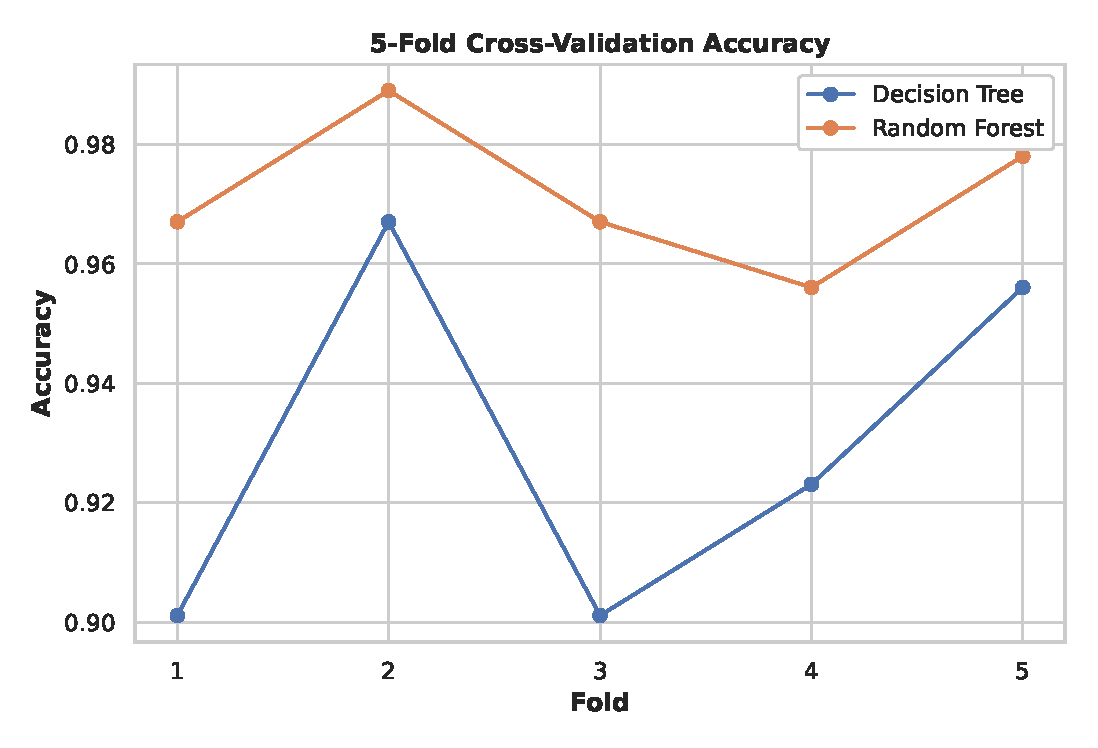
\includegraphics[width=\linewidth]{figures/5_fold_cv_comparison.eps}
\caption{5-Fold CV accuracy, per fold.}
\label{fig:cv_folds}
\end{minipage}\hfill
\begin{minipage}{0.48\linewidth}
\centering
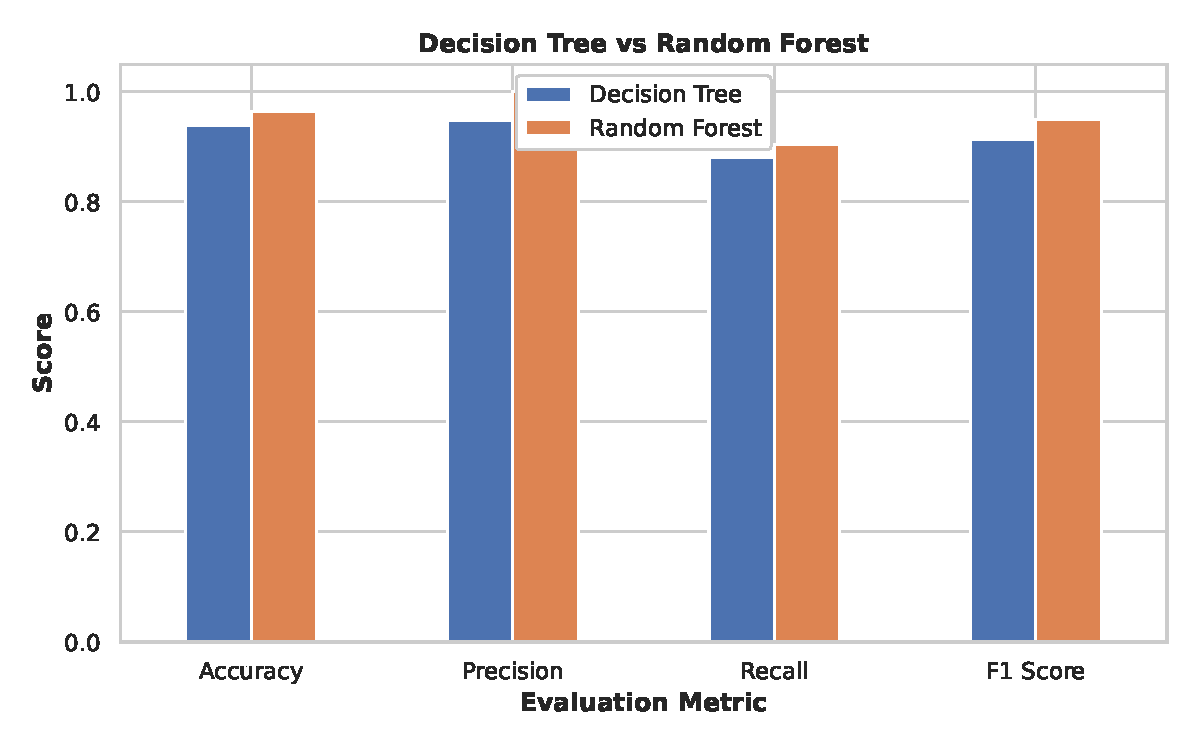
\includegraphics[width=\linewidth]{figures/model_metric_comparison.eps}
\caption{Test-set metric comparison.}
\label{fig:metric_bar}
\end{minipage}
\end{figure}
\textbf{Inference:} Random Forest wins every single fold in Figure~\ref{fig:cv_folds} (96.7 vs 90.1, 98.9 vs 96.7, 96.7 vs 90.1, 95.6 vs 92.3, 97.8 vs 95.6) -- not just on average, but on each one individually, which is honestly more convincing evidence of a real variance reduction than the average alone would be. The Decision Tree dipping to 90.1\% on folds 1 and 3, right next to a 96.7\% peak on fold 2, is a pretty clean example of the exact high-variance problem ensembling is supposed to fix. From Figure~\ref{fig:metric_bar}, the widest gap between the two models shows up in Precision (94.9\% $\to$ 100\%), while Recall barely moves (88.1\% $\to$ 90.5\%). So most of what Random Forest gains here seems to come from cutting down false alarms on the Benign class, rather than catching meaningfully more Malignant cases.
 
\begin{figure}[H]
\centering
\begin{minipage}{0.48\linewidth}
\centering
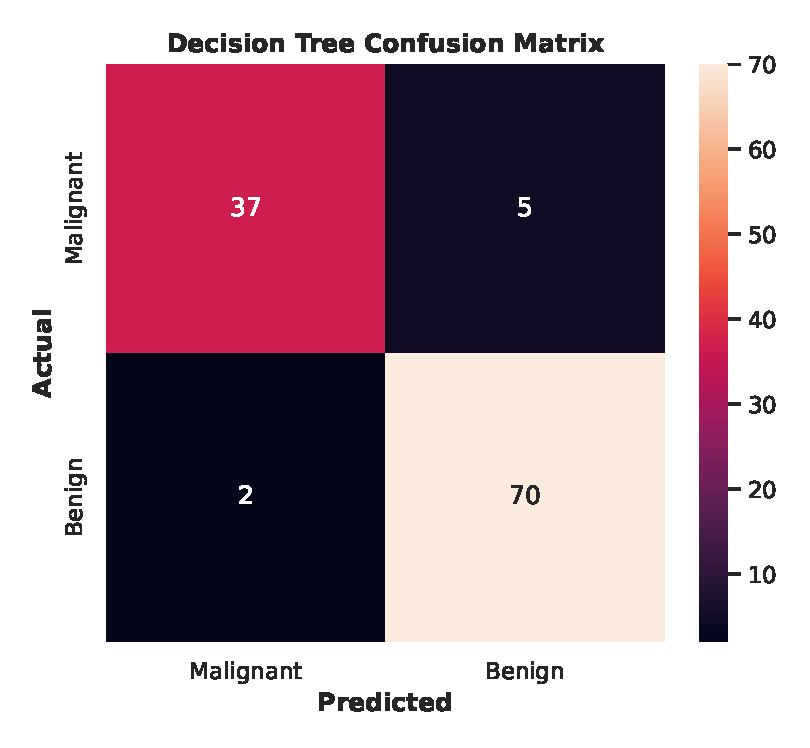
\includegraphics[width=\linewidth]{figures/decision_tree_confusion_matrix.eps}
\caption{Decision Tree confusion matrix.}
\label{fig:cm_dt}
\end{minipage}\hfill
\begin{minipage}{0.48\linewidth}
\centering
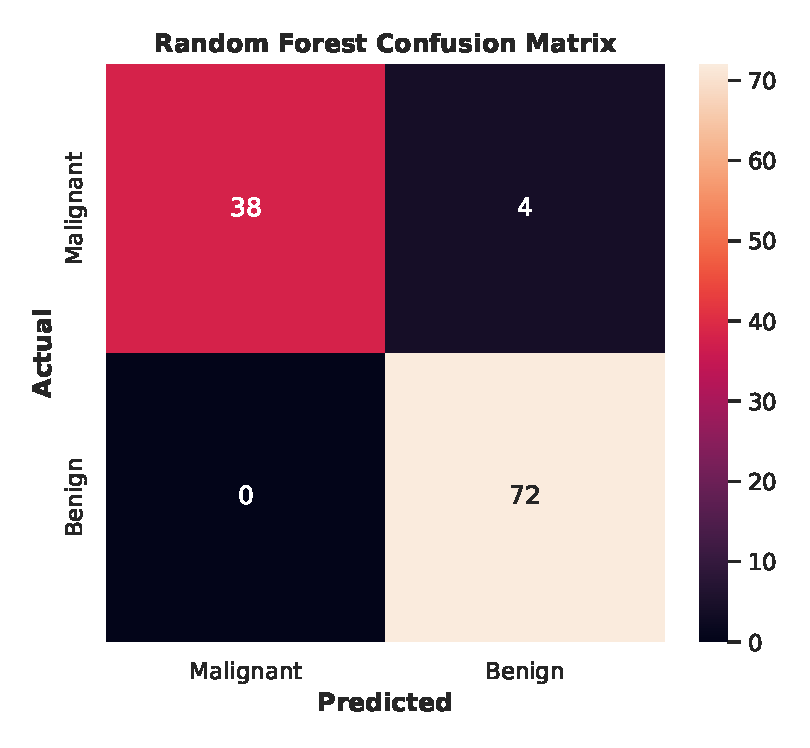
\includegraphics[width=\linewidth]{figures/random_forest_confusion_matrix.eps}
\caption{Random Forest confusion matrix.}
\label{fig:cm_rf}
\end{minipage}
\end{figure}
\textbf{Inference:} Out of 42 truly Malignant test cases, the Decision Tree misses 5 of them while Random Forest misses 4 (Figures~\ref{fig:cm_dt} and \ref{fig:cm_rf}). In a diagnostic setting, missing a cancer is a lot costlier than a false alarm, so recall on the Malignant class arguably matters more here than raw accuracy -- by that measure, neither model is where it needs to be, though Random Forest is marginally safer. On the Benign side, the Decision Tree wrongly flags 2 healthy cases as Malignant, while Random Forest gets all 72 right with zero false positives -- which is exactly what pushes its precision up to 100\%.
 
\begin{figure}[H]
\centering
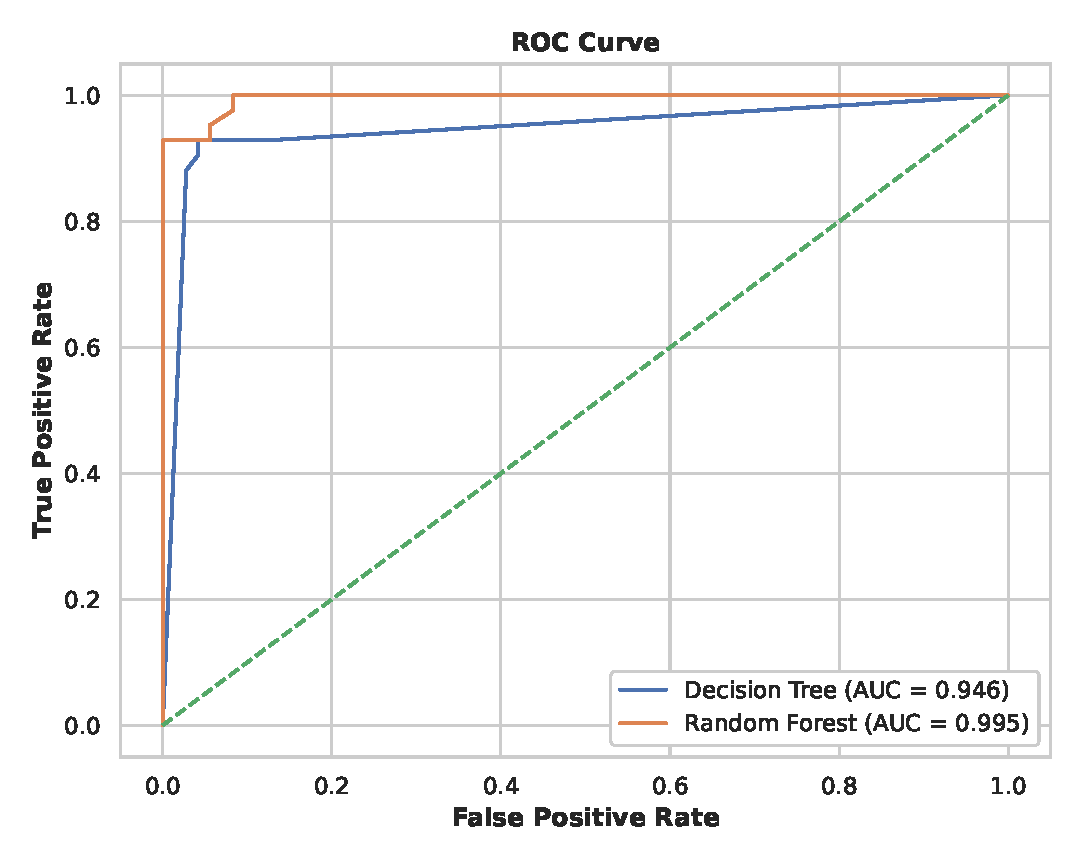
\includegraphics[width=0.62\linewidth]{figures/roc_curve.eps}
\caption{ROC curves for the tuned Decision Tree and Random Forest (Cell 25).}
\label{fig:roc}
\end{figure}
\textbf{Inference:} Both curves climb sharply toward the top-left corner and stay well clear of the diagonal, which lines up with the 94--96\% test accuracy both models posted. Random Forest (AUC = 0.995) sits above the Decision Tree (AUC = 0.946) at almost every threshold -- it reaches a true positive rate of 1.0 while the false positive rate is still under 0.1, whereas the Decision Tree's curve is noticeably more bowed and needs a higher false-positive rate to catch the same fraction of malignant cases. This lines up with what we already saw in the confusion matrices (Figures~\ref{fig:cm_dt}--\ref{fig:cm_rf}): Random Forest looks like the more reliable classifier across essentially the whole operating range, not just at the default 0.5 cutoff.

\section{Discussion}
A few things stood out beyond the headline accuracy numbers.
 
\begin{enumerate}
    \item \textbf{Ensembling helped, but tuning the Random Forest didn't -- at least not on this test split.} The \emph{default} Random Forest (100 trees, no tuning at all) scored 97.37\% test accuracy (Cell 26), while the grid-search-tuned version (\texttt{n\_estimators=50}, \texttt{max\_depth=10}, \texttt{bootstrap=False}) only managed 96.49\% (Cell 30) -- even though the tuned configuration was the one that won on 5-fold CV accuracy (97.14\%). We think this is a fairly direct illustration of the gap between cross-validation performance and a single held-out test set: the CV-selected hyperparameters generalised best \emph{on average across folds}, but that's no guarantee they'll beat every other configuration on one particular 114-sample test split. Interestingly, the Decision Tree went the other way -- tuning took it from 92.98\% (default) to 93.86\% (tuned) -- so "tuning always helps" held up for the high-variance model but not for the ensemble, which was already fairly stable to begin with.
    \item \textbf{For the Decision Tree, depth is really the knob that matters.} In the CV table, accuracy barely moves with \texttt{min\_samples\_split}/\texttt{min\_samples\_leaf} at a fixed depth -- it's flat at 92.09\% across all four leaf/split combinations when \texttt{max\_depth=3} -- but it shifts by up to 1.3 points when depth itself changes. Shallow trees (depth 3) underfit a little; the grid ended up choosing depth 7, which seems to balance bias and variance better than the shallower or deeper options we tried.
    \item \textbf{Random Forest's edge comes mostly from cutting false positives, not catching more true positives.} Precision jumped just over 5 points (94.9\% $\to$ 100\%), while recall moved by only 2.4 points (88.1\% $\to$ 90.5\%). For a cancer-screening use case, that means Random Forest is considerably better at not "crying wolf" on healthy patients, but only marginally better at catching every malignant case. Recall is really the metric that would need more work -- class-weighting, threshold tuning, maybe additional features -- before something like this could be trusted in an actual clinical pipeline.
\end{enumerate}

\section{Conclusion}
We trained a Decision Tree and a Random Forest on the 569-sample WDBC dataset and tuned both using 5-fold, stratified cross-validation. On the 114-sample held-out test set, the tuned Random Forest beat the tuned Decision Tree on every single metric (96.49\% vs 93.86\% accuracy, 95.00\% vs 91.36\% F1, 0.995 vs 0.946 AUC) -- and, more tellingly, it also won on \emph{every one of the five CV folds individually}, which matches the theoretical expectation that bagging plus random feature selection should reduce variance relative to a single tree. The ROC analysis backs this up across the full range of decision thresholds, not just at the default cutoff. One result worth carrying forward regardless of which model you pick: hyperparameter tuning chosen by CV accuracy doesn't automatically beat a default configuration on a single held-out split -- here, the untuned Random Forest actually scored higher on the test set (97.37\%) than the CV-tuned one did (96.49\%).

\section{References}
\begin{enumerate}
    \item W. N. Street, W. H. Wolberg, and O. L. Mangasarian, ``Nuclear feature extraction for breast tumor diagnosis,'' in \textit{IS\&T/SPIE Int. Symp. Electronic Imaging}, 1993. Dataset: \url{https://archive.ics.uci.edu/dataset/17/breast+cancer+wisconsin+diagnostic}
    \item L. Breiman, ``Random Forests,'' \textit{Machine Learning}, vol. 45, no. 1, pp. 5--32, 2001.
    \item Scikit-learn Developers, ``Decision Trees,'' \textit{scikit-learn documentation}. \url{https://scikit-learn.org/stable/modules/tree.html}
    \item Scikit-learn Developers, ``Ensemble methods -- Random Forests,'' \textit{scikit-learn documentation}. \url{https://scikit-learn.org/stable/modules/ensemble.html\#random-forests}
\end{enumerate}

\end{document}